\documentclass[12pt]{beamer}
\usepackage{beamerthemeHannover, graphicx, clrscode, amsmath, amssymb, multicol}
\usepackage{color, verbatim}
\setbeamercolor{sidebar}{use=structure,bg=gray!60!green}
\title{ A Visual Introduction To Parrot Virtual Machine }
\author[@dukeleto]{Jonathan "Duke" Leto \\ Community Manager \\ Parrot Virtual Machine \\ http://parrot.org }
\date{}

\begin{document}

\frame{
    \titlepage
    \begin{center}
        
\includegraphics[scale=0.5]{parrot_logo}
    \end{center}
}

\frame{
    \frametitle{ What is Parrot, really? }

    Parrot is many things:

    \begin{itemize}
        \item A culture
        \item A collection of languages
        \item A virtual machine to run said languages
        \item A set of tools to write new languages
        \item A playground for compiler + language research
        \item A second cousin to Perl 6
    \end{itemize}

    Parrot is what you want it to be.
}

\frame{
    \frametitle{ Parrot Culture }
    \begin{center}
     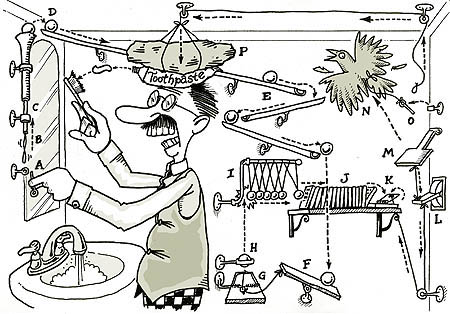
\includegraphics[scale=0.5]{rube-goldberg}
    \end{center}
}

\frame{
    \frametitle{ The Parrot Onion (NOW) }

    \begin{center}
     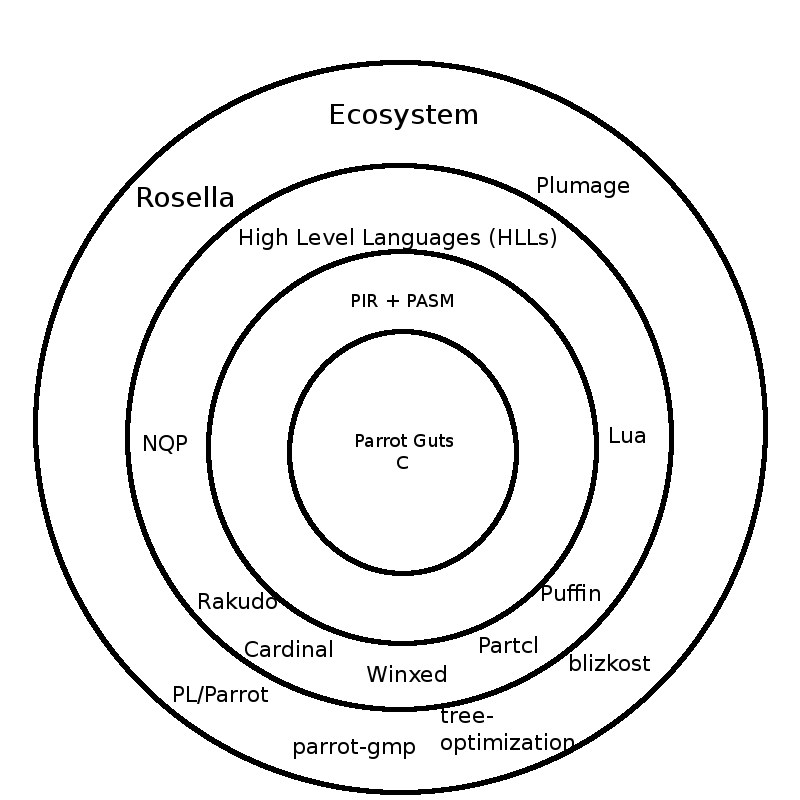
\includegraphics[scale=0.7]{parrot_onion}
    \end{center}
}

\frame{
    \frametitle{ The Future Parrot Onion }

    \begin{center}
     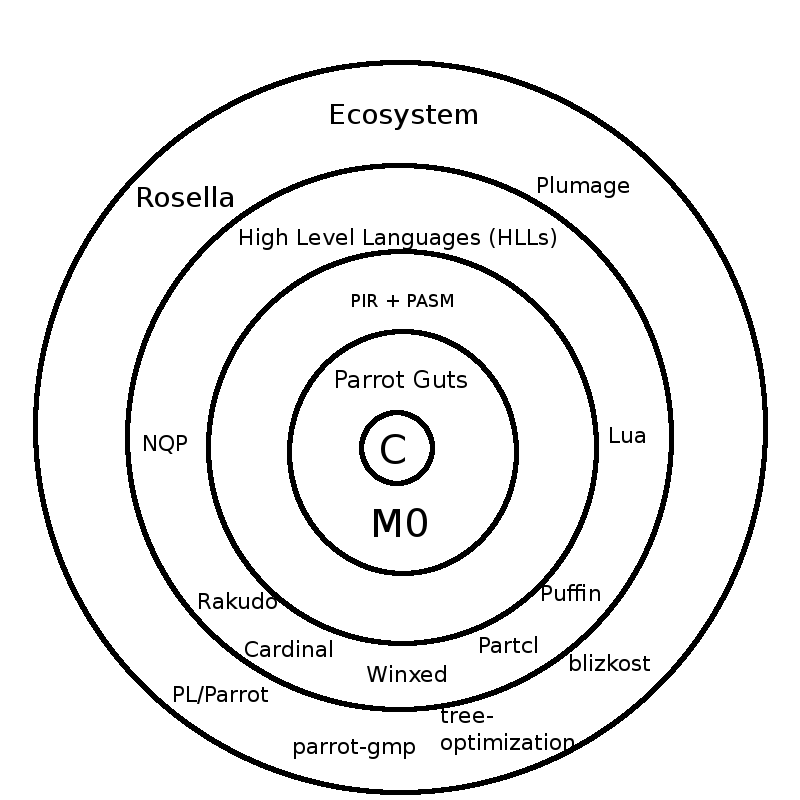
\includegraphics[scale=0.7]{parrot_onion_future}
    \end{center}

}

\frame{
    \frametitle{ PMC is for Cookie ... }
    PMC = Parrot Magic Cookie a.k.a. Objects \\
    Serious people prefer to call them PolyMorphic Containers, but not me

    \begin{center}
     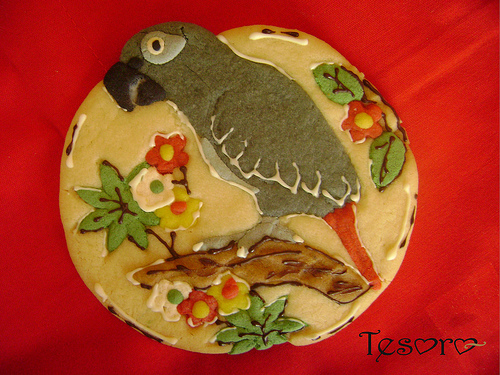
\includegraphics[scale=0.4]{parrot_cookie}
    \end{center}
}

\frame{
    \frametitle{ PMC is for Cookie ... }

    Meta-recipe:
    \begin{center}
        \begin{itemize}
            \item \_ cups of \_ flour
            \item \_ \_ eggs
            \item \_ cups of \_ chocolate chips
            \item \_ cups of \_ sugar
            \item \_ sticks of \_ butter
            \item \_ spoons of \_ butter
        \end{itemize}
    \end{center}

}

\frame{
    \frametitle{ PMC is for Cookie ... }

    Some people like really sweet, dark chocolate chip, peanut butter cookies.

    \begin{center}
        \begin{itemize}
            \item \underline{2} cups of \underline{white} flour
            \item \underline{2 organic} eggs
            \item \underline{1} cup of \underline{dark} chocolate chips
            \item \underline{3} cups of \underline{cane} sugar
            \item \underline{2} sticks of \underline{unsalted} butter
            \item \underline{3} spoons of \underline{peanut} butter
        \end{itemize}
    \end{center}

}

\frame{
    \frametitle{ PMC is for Cookie ... }

    OH NOES! Some people are allergic to peanut butter, dislike processed flour
    and prefer milk chocolate!  Also, almond butter is a delicious replacement
    for peanut butter.

    \begin{center}
        \begin{itemize}
            \item \underline{2} cups of {\color{red} \underline{wheat}} flour
            \item \underline{2 organic} eggs
            \item \underline{1} cup of {\color{red} \underline{milk}} chocolate chips
            \item \underline{3} cups of \underline{cane} sugar
            \item \underline{2} sticks of \underline{unsalted} butter
            \item \underline{3} spoons of {\color{red} \underline{almond}} butter
        \end{itemize}
    \end{center}

}

\frame{
    \frametitle{ The meta-recipe is actually a VTABLE! }

    VTABLE = virtual tables \\

    Examples of actual VTABLEs:\\
    \begin{center}
        \begin{itemize}
            \item get\_integer - get integer representation of PMC
            \item set\_integer - set integer representation of PMC
            \item get\_number - get numeric/float representation
            \item set\_number - set numeric/float representation
            \item elements - get the number of elements
        \end{itemize}
    \end{center}

    Just like no recipe uses every ingredient in your fridge, each PMCs does not implement every VTABLE.
}

\frame{
    \frametitle{ Register-based }

    No stacks! Like Lua VM and Dalvik VM

    \begin{center}
        
\includegraphics[scale=1.0]{stacks}
    \end{center}

    Different set of optimizations than stack-based VMs
}

\frame{
    \frametitle{ Continuation Passing Style }

    Keep passing it along...

    \begin{center}
        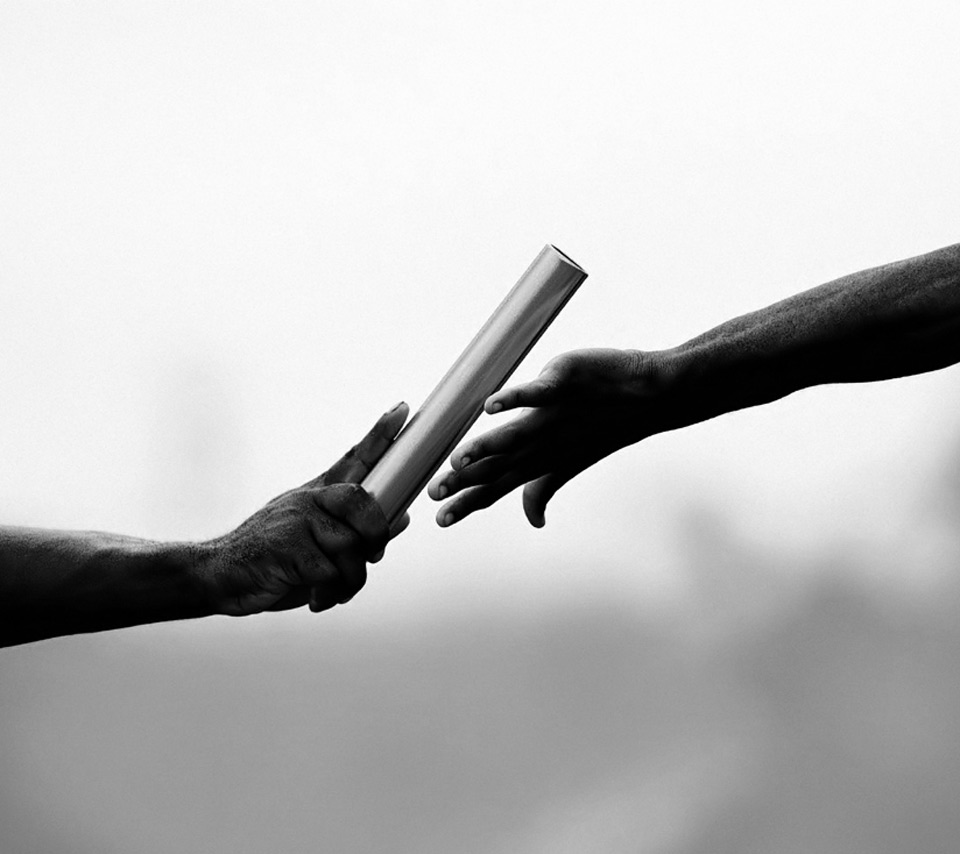
\includegraphics[scale=0.2]{cps}
    \end{center}
}


\frame{
    \frametitle{ Deprecation Policy }

    We give our APIs a bath every three months...

    \begin{center}
        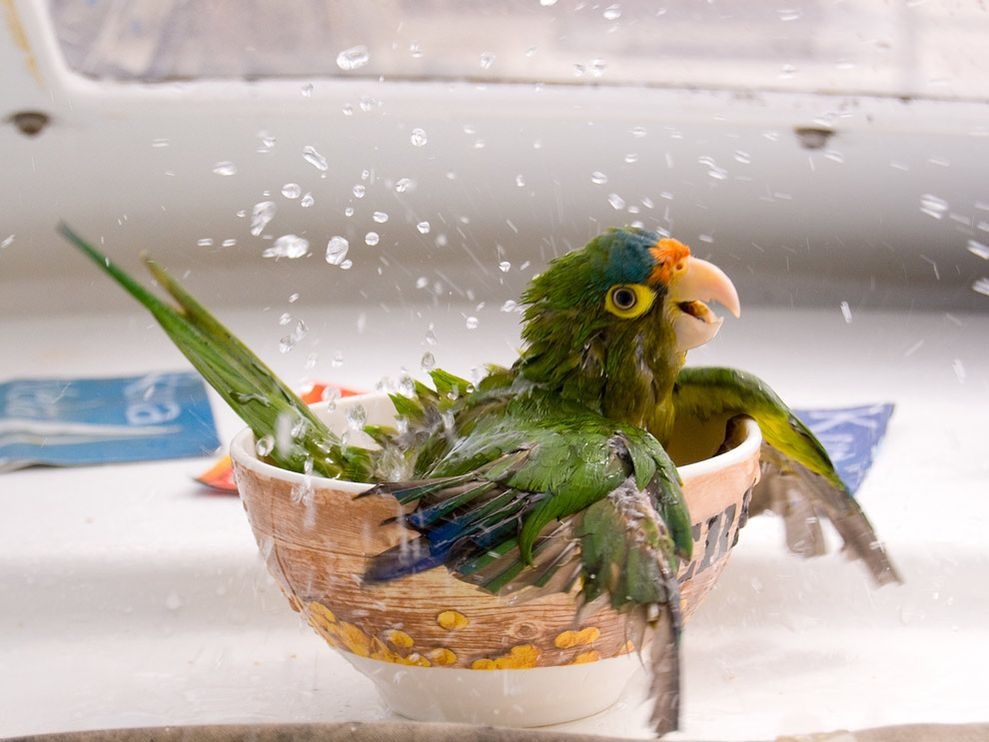
\includegraphics[scale=0.2]{parrot_bath}
    \end{center}
}

\frame{
    \frametitle{ Deprecation Policy }

    api.yaml

    \begin{center}
        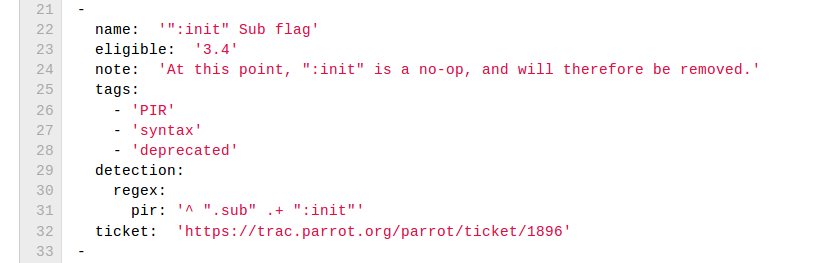
\includegraphics[scale=0.3]{api_yaml}
    \end{center}

    tools/dev/show\_deprecated.nqp \\
    tools/dev/resolve\_deprecated.nqp \\
    tools/dev/show\_experimental.nqp \\
    tools/dev/dedeprecator.nqp \\
}

\frame{
    \frametitle{ Parrot Compiler Toolkit (PCT) }

    We give you the dough, you cook it...

    \begin{center}
        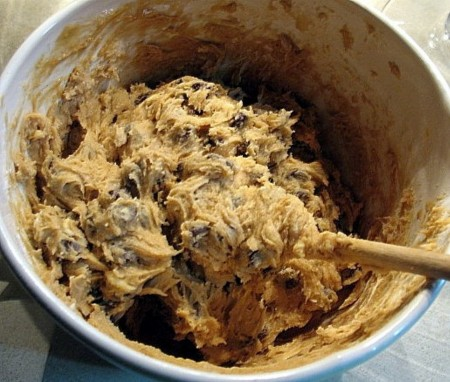
\includegraphics[scale=0.4]{cookie_dough.jpg}
    \end{center}
}

\frame{
    \frametitle{ Parrot Compiler Toolkit (PCT) }

    Web Interface Coming Real Soon Now
    \begin{itemize}
        \item tools/dev/mk\_language\_shell.pl - PIR build system
        \item tools/dev/create\_language.pl    - Perl 5 build system \\
    \end{itemize}
}

\frame{
    \frametitle{ Resources }
    \begin{center}
        \begin{itemize}
            \item http://docs.parrot.org
            \item \#parrot on irc.parrot.org
            \item parrot-dev and parrot-users mailing lists
            \item https://github.com/Benabik/cish
        \end{itemize}
    \end{center}
}

\frame{
    \frametitle{ Thanks! }
    \begin{center}
        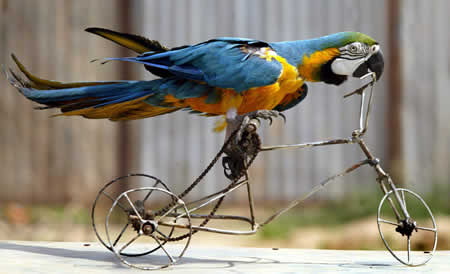
\includegraphics[scale=0.4]{thanks.jpg}
    \end{center}

    Slides at https://github.com/leto/presentations

}

\end{document}
